\section{受条款约束的保障机制的参考设计}
\label{sec:design}

证据表明，类型化决策模型在诸如 \pol{} 安全阀这样的保障机制中可承担的合理角色是：一个快速、低成本、留有记录的\emph{检测器}，而非\emph{裁决者}。
\Cref{fig:architecture} 勾勒了一个基于这一原则、针对 \clause{5.4.1} 安全阀的设计；它适用于任何对 AI 系统的输入和输出进行筛查的治理层。
它与 NaturalDAO 治理工作组的试点协议相兼容；作者参与该工作组，该协议已区分 \texttt{conforming}、\texttt{violating} 与 \texttt{insufficient} 三种判定，以及放行、修复、阻断、澄清与复核五种动作~\cite{polgov}；本设计增加了临时性的\emph{暂扣}，并规定\emph{阻断}仅在人工确认后方为最终决定。
凡某项建议与该协议中已作出的选择相一致之处，我们均予以说明，以便读者判断推动该建议的是证据还是先前的设计。

\begin{figure}[t]
\centering
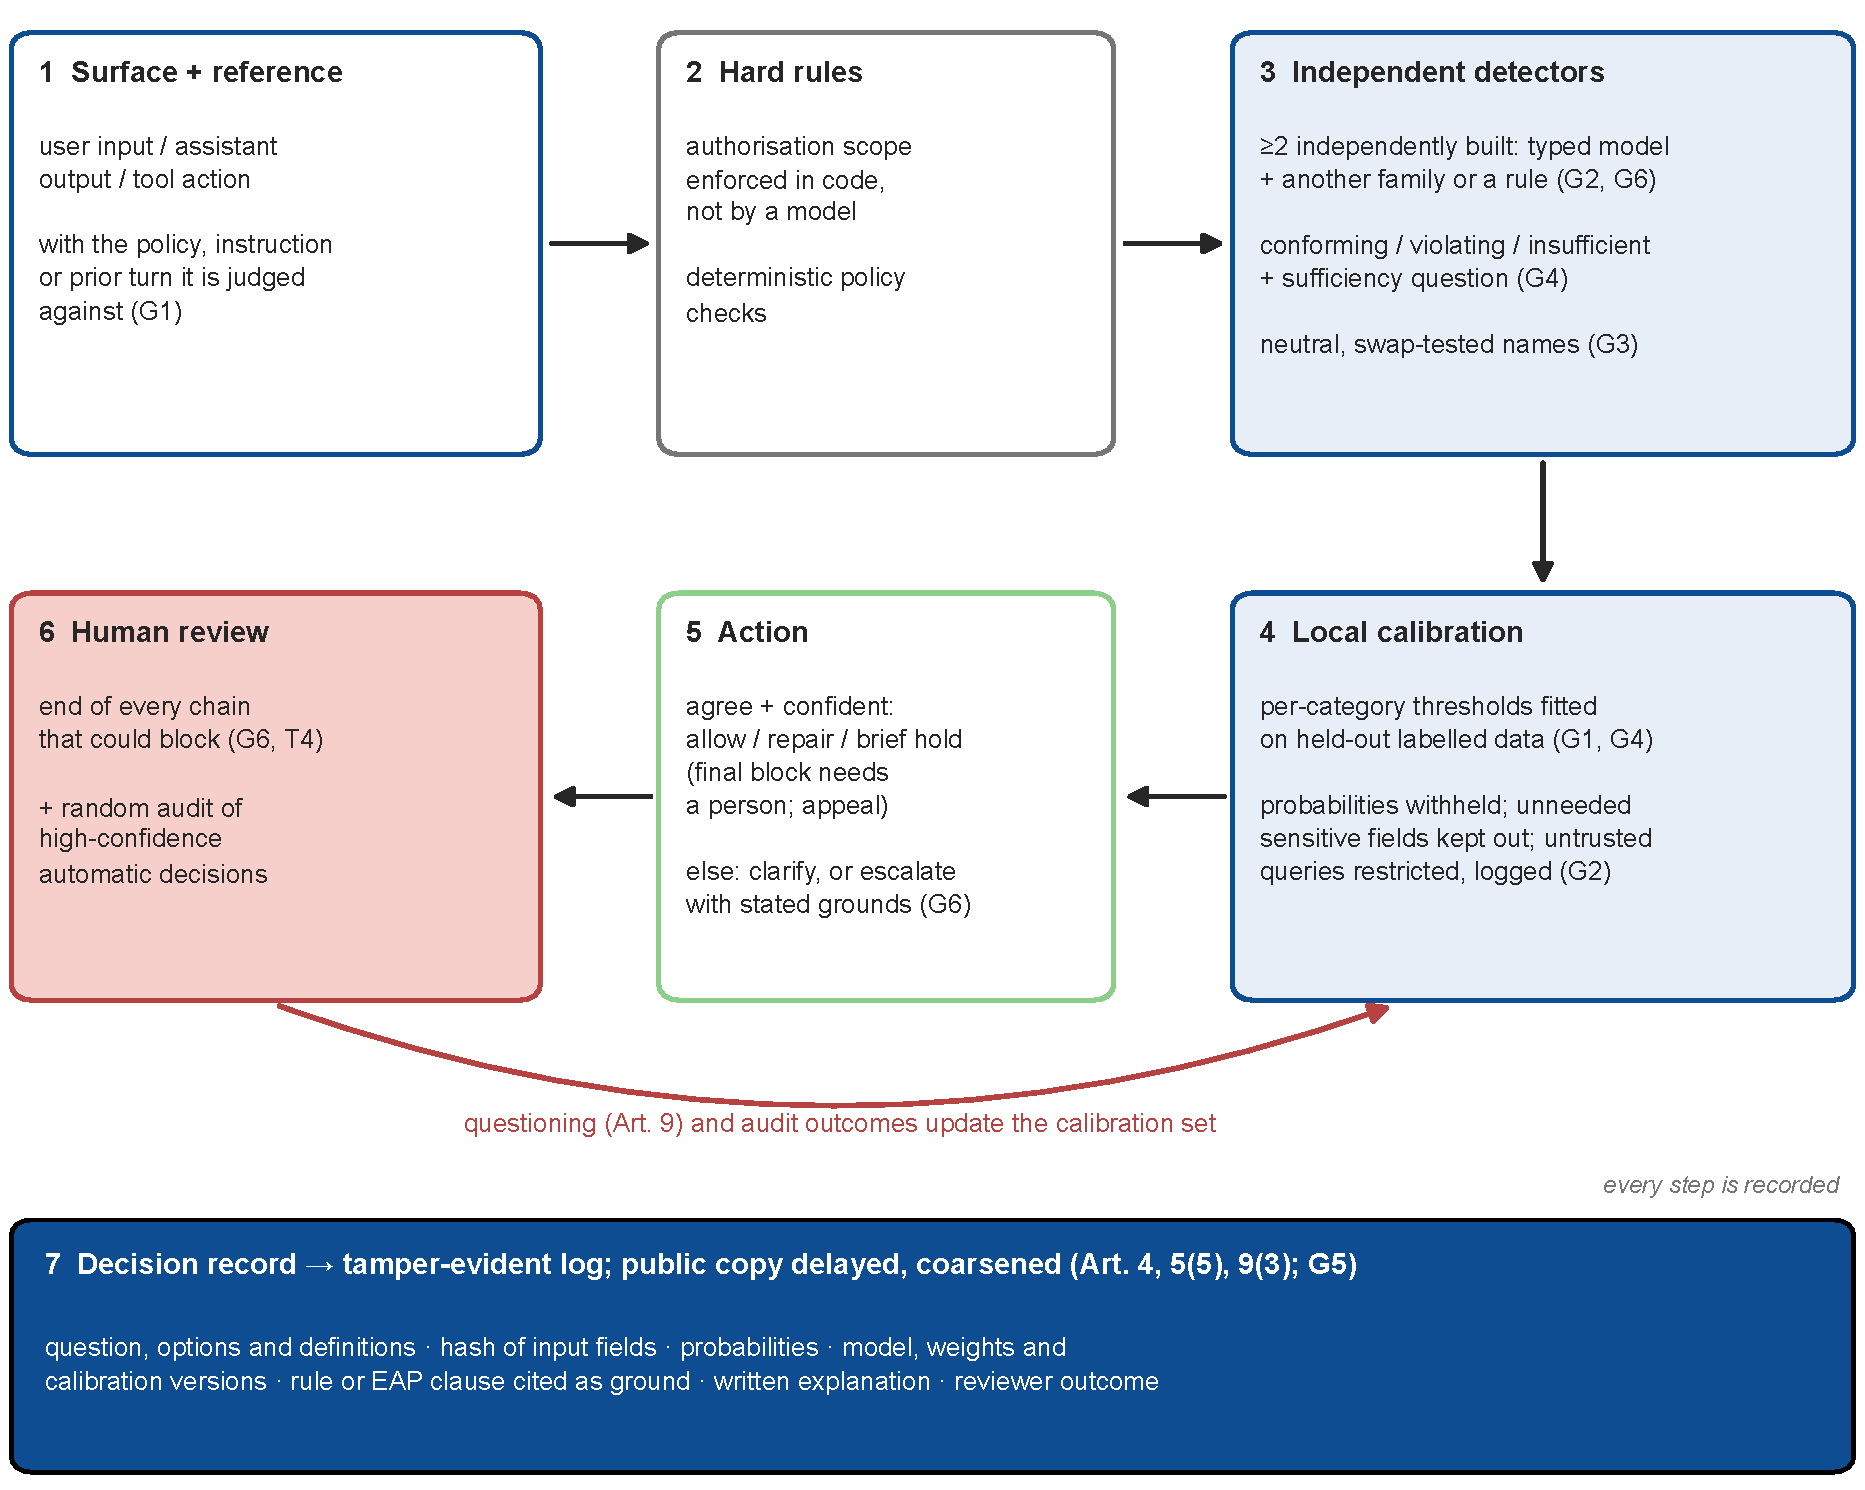
\includegraphics[width=0.8\linewidth]{figures/fig_architecture.pdf}
\caption{受条款约束的安全阀的参考设计。类型化模型作为检测器（3），其输出在任何自动动作（5）之前先经本地校准（4）；分歧与信息不足的情形予以澄清或升级，任何最终阻断均由人确认，高置信自动决策的随机样本由人审计（6）；每一步均写入决策记录（7）。括号中的标签给出促成各要素的要求或张力。}
\label{fig:architecture}
\end{figure}

该设计包含七个要素。
\begin{enumerate}
  \item \textbf{向检测器提供参照，而不仅是文本。} 许多失效是相对于某条指令、某项政策或某个先前陈述而界定的~\cite{arx29429}；受审内容始终与该语境配对提供。需要计算或推理的事实（求和、日期、后果）在代码中或在单独记录的步骤中计算并写入状态，而不交给检测器~\cite{arx39496,arx01834}。
  \item \textbf{在代码中强制执行权限范围。} 智能体是否停留在其授权范围之内，是外围系统的属性~\cite{arx22664}，应在调用任何模型之前通过能力检查强制执行。
  \item \textbf{使用至少两个独立构建的检测器。} 阻断信号要求构造不同的检测器之间取得一致，例如不同模型家族的模型，或一个模型与一条规则，因为同类模型会共享高置信错误~\cite{arx29769}；而与一条不同构造的规则取得一致，使审核者能够跳过约三分之一的案例而不损失 macro-F1，尽管被标记为非良性的伪装攻击有所减少~\cite{arx02048}。每个问题都是三值的（符合、违反、信息不足），充分性也作为单独的是/否问题提出~\cite{arx01006}，选项使用绑定到定义的中性标识符，并须通过重命名测试~\cite{arx26758,arx00346}。必须相互独立失效的标记（放行/阻断、风险等级、是否需要人工）在不同的调用中分别询问，因为在一个与 \jev{} 兼容的开源模型中，一条植入的注释就改变了同一调用中的多个答案~\cite{zen23038928}\zmark{}。在准确性足够之处，优先使用可自托管的模型（T3）。三值判定已是该工作组试点协议的一部分。
  \item \textbf{本地校准，不向不受信任的调用方提供概率，并限制其可查询的内容。} 阈值按类别在留出的本地数据上拟合~\cite{arx29429,arx24052,jkf87_2026replication}，在可交换性假设合理之处采用无分布风险控制~\cite{bates2021distribution,angelopoulos2024conformal}，并对每种新的问题类型重新认证~\cite{arx33689}，同时按既定时间表定期重新认证，且每当时间再验证未通过时（\cref{tab:checklist} 第~16 项）亦予重新认证。原始概率不返回给不受信任的调用方，因为概率有助于攻击者优化攻击，尽管仅凭标签攻击也能得逞~\cite{arx30243,arx28613}；决策所不需要的字段，尤其是敏感属性，不放入检测器的输入，因为一名获得该任务授权的用户通过在输入中植入条件指令，仅凭标签、每个状态两至六次查询即恢复了隐藏属性；不受信任的调用方的查询限于经授权的任务，因为标签曾被用来完善有害计划，且这些查询须予记录，因为标签还曾被用来训练替身模型~\cite{arx04985}。
  \item \textbf{仅在取得一致时自动行动，且对人的限制只能是短暂和可逆的。} 一致加上经过校准的置信度，允许自动\emph{放行}、自动\emph{修复} AI 系统自身的输出（例如 \clause{4.3.3.1} 的恨语截断，但绝不编辑人的消息），以及对人的内容进行有时限（例如至多 24 小时）且完全可逆的\emph{暂扣}。暂扣只有经人确认后，才成为对某人言论、某项福利或某个账户的最终阻断，并始终可以申诉。出现分歧或 \texttt{insufficient} 时，转入澄清，或升级至一个必须陈述其依据的更强推理模型~\cite{arx26550}。由于自动放行对任何受被放行内容伤害的人都具有实质后果，漏检率与误阻断率一并受到监测与治理。正是这一要素使类型化模型保持在\cref{sec:intro} 意义上的检测器角色。
  \item \textbf{每一条可能导致阻断的链路都以人为终点，并审计高置信决策。} 审核者查看每一项将以阻断告终的升级、每一项未解决的升级，以及高置信自动决策的随机样本，因为危害最大的错误是高置信且共享的~\cite{arx29769,arx33401}；审核结果以及依 \art{9} 进行的公众质询的结果，回馈到校准集中。
  \item \textbf{记录每一项决策。} 每条记录包含问题、选项集合与定义、输入字段的哈希值、概率、模型版本、权重版本与校准版本、作为依据援引的规则或条款、任何书面解释，以及审核者的处理结果。记录保存在向监督者开放的防篡改日志中（\art{9}(3)）；公开版本以粗化并延迟的方式发布概率，从而服务于 \art{4} 与 \art{5}(5)，而不致成为攻击者可反复试探的判定接口（oracle）。
\end{enumerate}

\paragraph{使人工复核切实可行。}
链路终点上的人只有在能够胜任这项工作时，才构成保障机制。
审核者需要容量：严格的错误上限会把工作量转移到复核与阻断上~\cite{arx33401}，插入的观点会把高置信答案推入复核~\cite{arx31142}，因此复核负荷必须与准确性一并纳入预算并予以报告，而更低成本的评估可能增加而非减少总负荷~\cite{arx01231}。
审核者容易产生自动化偏差与自满~\cite{parasuraman2010complacency,green2022flaws}，并可能成为系统失效责任的落脚点~\cite{elish2019moral}，因此在随机审计期间应隐藏模型的判定与概率，并测量审核者之间的一致性，而不仅是其与模型的一致性。
人们也恰恰在类型化模型最过度自信的那些有争议条目上意见分歧~\cite{pavlick2019inherent,davani2022dealing,zen23032384}\zmark{}，因此有争议的类别需要不止一名审核者，而受影响的人需要得到通知、理由说明和申诉途径~\cite{santaclara2021,dsa2022}。

\paragraph{本设计的权衡与已知局限。}
要求两个检测器在阻断前取得一致会降低灵敏度：更多违规会被漏检，这与通常靠更多阻断来满足的严格漏检上限相冲突~\cite{arx33401}；本设计转而接受更多暂扣与更多复核，其漏检率必须加以测量。
风险控制的保证以校准数据与部署数据之间的可交换性为前提；它们在良性漂移下而非自适应攻击下约束错误，而 G2 的证据表明自适应攻击是现实的。
就仇恨言论而言，这种分布偏移并非假设：在 20 个语言模型上，四个静态英文仇恨言论基准上的排名并不能预测其在带时间戳数据或新词替换数据上的排名（Spearman $\rho$ 介于 $-0.31$ 与 $0.19$ 之间，所有 90\% 区间均包含零），而各静态基准彼此之间相互一致（平均 $\rho = 0.36$）~\cite{dibonaventura2025hatevolution}。
为独立标记分别调用以及增加第二个检测器，会成倍增加成本与延迟，削弱类型化模型的主要优势，尽管已测得的成本留有很大余地~\cite{arx00346,arx01079}。
最后，大多数要素所依据的证据确定性为低或极低（见\cref{tab:keyfindings}）；本设计是一个有待在 \pol{} 的构念上检验的假设，而非经过验证的系统。

\Cref{tab:checklist} 将证据转化为一份核查清单，适用于任何拟用于此类保障机制的类型化模型。
第 1--4、9、14 和 15 项借鉴了~\cite{arx32160} 的 14 项中的 9 项（其 B1--B2、C1、C3--C4、R1--R2 与 T2--T3）；其余各项为治理保障机制而增设，该清单的 B3、T1、T4、R3 与 C2 未予采用。每一项都有一个暂定的通过标准；这些数值是供部署该保障机制者设定的起点，而非经实证验证的阈值。

\begin{table}[!htbp]
\centering
\footnotesize
\caption{用于治理保障机制中类型化决策模型的评估核查清单及暂定通过标准。“依据”给出相应的证据或条款；标有 $\circ$ 的条目是在~\protect\cite{arx32160} 的核查清单之外增设的。}
\label{tab:checklist}
\begin{tabularx}{\linewidth}{@{}rL>{\raggedright\arraybackslash}p{0.27\linewidth}>{\raggedright\arraybackslash}p{0.17\linewidth}@{}}
\toprule
\# & 要求 & 暂定通过标准 & 依据 \\
\midrule
1 & 与生成式模型的标签概率读出以及低成本生成式级联进行比较 & 在相同条目上报告 & \cite{arx32160} \\
2 & 在留出的本地数据上拟合阈值；报告拟合阈值与默认阈值下的 F1 & 拟合阈值以单侧风险界加以认证 & \cite{arx29429,arx00346} \\
3 & 按类别报告本地重新校准前后的校准情况 & 按类别报告 ECE 与斜率及其区间 & \cite{arx24052,arx27607} \\
4 & 选项名称互换测试 & 定义互换下的翻转率至多为重复噪声下限的两倍 & \cite{arx26758,arx00346} \\
5$^\circ$ & 包括 \texttt{insufficient} 在内的三个选项，外加单独的充分性问题 & 在成对的信息存在/缺失条目上，\texttt{insufficient} 的召回率至少为 0.5 & \cite{arx39496,arx01006,polgov} \\
6$^\circ$ & 互补问题与互斥问题的一致性 & 与总和为一的偏差在重复噪声的两倍以内 & \cite{arx33209} \\
7$^\circ$ & 以自适应的概率引导式添加、插入观点、诱饵与多轮攻击进行红队测试，并在已部署的输入与查询限制下进行仅凭标签的判定接口（oracle）攻击（属性推断、替身模型提取） & 按攻击类型报告攻击成功率，且低于预先设定的目标 & \cite{arx30243,arx31142,arx01834,checkpoint2026jev,arx04985} \\
8$^\circ$ & 按子类型（包括高置信错误）分解错误 & 没有召回率低于设定下限的子类型 & \cite{arx33401} \\
9 & 跨重复、接口与分解方式的决策层面稳定性 & 报告跨接口的分歧；每个问题固定一种接口 & \cite{arx27678,arx37470,arx33971} \\
10$^\circ$ & 与每个升级目标之间的错误相关性 & 高置信错误的重复率低于独立情形加上设定余量 & \cite{arx29769} \\
11$^\circ$ & 以中文及所服务的每种语言进行评估，并包含文字与选项顺序变体 & 每种语言均在英文的设定余量之内 & \cite{qin2026zhdecisionbench,typesafe_models} \\
12$^\circ$ & 不在人群之间进行强制选择；对行为问题进行群体偏见测试 & 各群体的错误率在设定余量之内 & \cite{simmons2026saidno,sap2019risk} \\
13$^\circ$ & 价值负载问题：无人设时的默认立场，以及在人们意见分歧处的表现 & 予以报告；有争议条目交由人处理 & \cite{arx36399,zen23032384} \\
14 & 有无缓存时的延迟；每个正确决策的成本 & 予以报告，包括复核负荷 & \cite{arx32160,arx00346} \\
15 & 版本与可检查性 & 在每条记录中固定模型、权重与校准版本；可自托管或留有记录 & \art{4}、\art{5}(4)--(5)、\clause{5.5} \\
16$^\circ$ & 时间再验证：在由近期条目构成的带时间戳留出集上，以及在将目标词替换为新近出现的同义新词的成对条目上重新评估 & 在所服务的每种语言中（第 11 项）：恨语的分时段召回率在认证时段的设定余量之内，且新词替换句对上的翻转率在重复噪声下限的设定余量之内；任一项超出时，按第 2 项的程序重新认证阈值 & \cite{dibonaventura2025hatevolution}（仅英文；未测试类型化模型） \\
\bottomrule
\end{tabularx}
\end{table}
